\documentclass[conference]{IEEEtran}
\usepackage{times}

% numbers option provides compact numerical references in the text.
\usepackage[numbers]{natbib}
\usepackage{multicol}
\usepackage[bookmarks=true]{hyperref}

\usepackage{graphicx} % more modern
%\usepackage{epsfig} % less modern
\usepackage{subfigure}

% For algorithms
\usepackage{algorithm}
\usepackage{algorithmic}
\usepackage{amsmath}
\usepackage{amssymb}
% Include other packages here, before hyperref.
\usepackage{color}
\usepackage{setspace}
\usepackage{wrapfig}
\usepackage{dsfont}

\usepackage[it,small]{caption}


\newcommand{\argmax}{\operatorname{arg\,max}}
\newcommand{\argmin}{\operatorname{arg\,min}}
\newcommand{\todo}[1]{\textcolor{blue}{\textbf{#1}}}
\newtheorem{mydef}{Definition}



\graphicspath{{./images/}}
\usepackage{multirow}
% Some illegal space-saving macros
%  \parskip=5pt
%  \abovedisplayskip 3.0pt plus2pt minus2pt%
% \belowdisplayskip \abovedisplayskip
% \renewcommand{\baselinestretch}{0.97}



\newenvironment{packed_enum}{
\begin{enumerate}
  \setlength{\itemsep}{0pt}
  \setlength{\parskip}{0pt}
  \setlength{\parsep}{0pt}
}
{\end{enumerate}}

\newenvironment{packed_item}{
\begin{itemize}
  \setlength{\itemsep}{0pt}
  \setlength{\parskip}{0pt}
  \setlength{\parsep}{0pt}
}{\end{itemize}}


 \newlength\savedwidth
 \newcommand\whline[1]{\noalign{\global\savedwidth\arrayrulewidth
								\global\arrayrulewidth #1} %
					   \hline
					   \noalign{\global\arrayrulewidth\savedwidth}}
 \renewcommand\multirowsetup{\centering}


\newlength{\sectionReduceTop}
\newlength{\sectionReduceBot}
\newlength{\subsectionReduceTop}
\newlength{\subsectionReduceBot}
\newlength{\abstractReduceTop}
\newlength{\abstractReduceBot}
\newlength{\captionReduceTop}
\newlength{\captionReduceBot}
%\newlength{\nameReduceTop}
\newlength{\subsubsectionReduceTop}
\newlength{\subsubsectionReduceBot}

\newlength{\horSkip}
\newlength{\verSkip}

\newlength{\figureHeight}
\setlength{\figureHeight}{1.7in}

%\newlength{\figureFraction}
\setlength{\horSkip}{-.09in}
\setlength{\verSkip}{-.1in}
%\setlength{\figureFraction}{.195}


%
\setlength{\subsectionReduceTop}{-0.05in}
\setlength{\subsectionReduceBot}{-0.15in}
\setlength{\sectionReduceTop}{-0.07in}
\setlength{\sectionReduceBot}{-0.1in}
\setlength{\subsubsectionReduceTop}{-0.06in}
\setlength{\subsubsectionReduceBot}{-0.05in}
%
%
%\setlength{\figureHeight}{1.5in}
\setlength{\abstractReduceTop}{-0.10in}
\setlength{\abstractReduceBot}{-0.05in}
%
%

%\setlength{\nameReduceTop}{-0.05in}


\setlength{\captionReduceTop}{-0.15in}
\setlength{\captionReduceBot}{-0.15in}



\pdfinfo{
   /Author (Homer Simpson)
   /Title  (Robots: Our new overlords)
   /CreationDate (D:20101201120000)
   /Subject (Robots)
   /Keywords (Robots;Overlords)
}

\usepackage{helvet}
%\renewcommand{\familydefault}{\sfdefault}

\begin{document}


% paper title
\title{Supplementary Material For \\ rCRF: Recursive Belief Estimation over CRFs in RGB-D Activity Videos}

% You will get a Paper-ID when submitting a pdf file to the conference system
%\author{Author Names Omitted for Anonymous Review. Paper-ID 63}
\author{
\authorblockN{Ozan Sener}
\authorblockA{School of Electrical \& Computer Eng. \\ Cornell University}
\and
\authorblockN{Ashutosh Saxena}
\authorblockA{Department of Computer Science \\ Cornell University}
}


\maketitle

\IEEEpeerreviewmaketitle

\section{Re-defining the belief}
\begin{figure}[h!]
  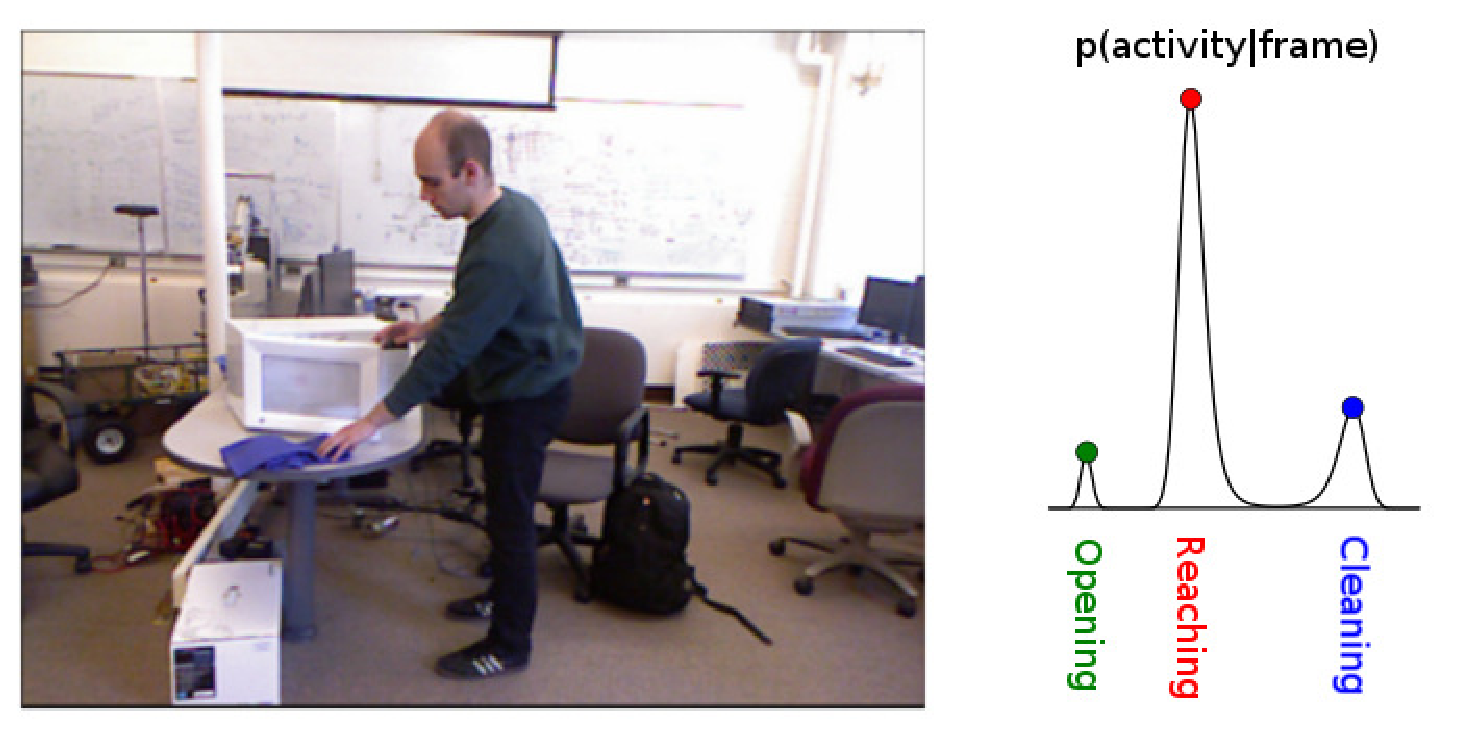
\includegraphics[width=\linewidth]{fig2}
  \caption{\textbf{Typically there are only a few plausible explanations per scene}. For this scene, only \emph{cleaning the table}, \emph{reaching to the cloth}, \emph{reaching to the microwave}, \emph{opening the microwav} are plausible.
}
\end{figure}

\textbf{\emph{CRF-likelihood over a natural scene concentrates on a few plausible samples!}}
\vspace{5mm}

We compute the belief for only the plausible samples as;
\begin{equation}
  \text{approx\_bel}^t(\mathbf{y})=\left\{ \begin{array}{cc} \frac{bel^t(\mathbf{y})}{\sum_{\mathbf{y}^\prime \in \mathbf{Y}^t} bel^t(\mathbf{y}^\prime)} & \text{if $\mathbf{y} \in \mathbf{Y}^t$} \\ 0 & \text{o.w.} \end{array} \right.
\end{equation}

where the set of plausible solutions at time $t$ is \mbox{$\mathbf{Y}^t={\mathbf{y}^{t,1},\ldots,\mathbf{y}^{t,M}}$}.

\section{How to find these samples?}
\textbf{Observations:}
\begin{itemize}
\item These samples have high likelihood since they are plausible
\item These samples are diverse because there are likely solutions around MAP solutions (eg. small perturbation of the MAP solution)
\end{itemize}

\textbf{Formulation:} We solve the following optimization problem in order to get the plausible solutions (we use hamming distance as $\Delta$ in our experiments);
\begin{equation}
\begin{aligned}
\mathbf{y}^{t,i} &= \argmax_{\mathbf{y}}  bel^t(\mathbf{y}) \\
&s.t.\,\, \Delta(\mathbf{y},\mathbf{y}^{t,j}) \geq \delta \quad \forall \; {j < i}
\end{aligned}
\label{divopt}
\end{equation}
%where $\bf{y}^{t,i}$ is the $i^{th}$ sample in the $t^{th}$ frame.


\end{document}
